In the analyses with exactly one lepton, three separate searches are performed.
In the first search, a search for direct stop pair production~\cite{1lstop2015}, the signal region is defined by having
exactly 1 lepton, at least 2 jets with at least one of the jets passing the criteria to be tagged as a b-jet, and \MET\ $>$ 250 GeV.
After these cuts are made, the largest background comes from SM \ttbar\ to dilepton where one of the leptons is lost leading to increased \MET\ in the event.
The results of this analysis increase the sensitivity to stop production for signal models with a stop mass of 750 GeV,
which is an improvement on the previous result which was sensitive to models with a stop mass up to 650 GeV.
%% The yields in data overlaid on the background predictions can be seen on the left in figure~\ref{fig:1lstopresults},
%% and the cross section upper limit is shown as a function of the stop mass on the x-axis and LSP mass on the y-axis.

%% \begin{figure}[!htb]
%% \begin{center}
%% \begin{tabular}{cc}
%% 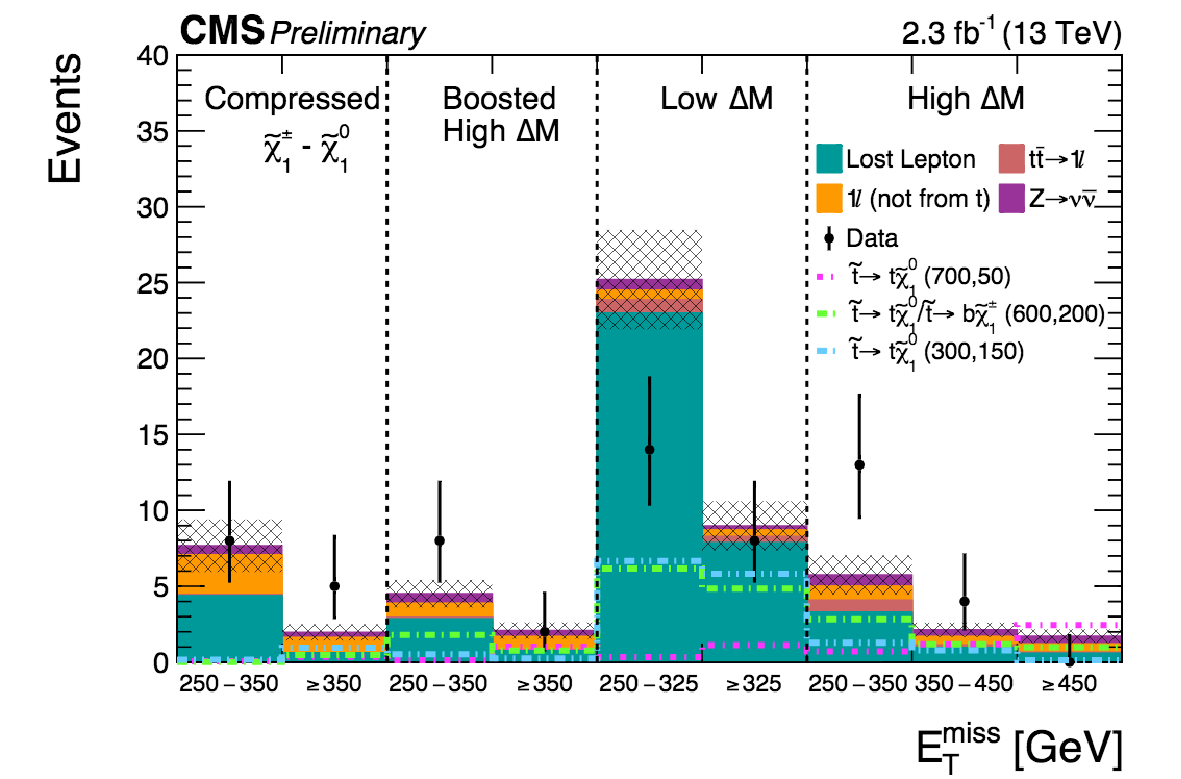
\includegraphics[width=0.4\textwidth]{1lstop/results_summary.pdf} &
%% 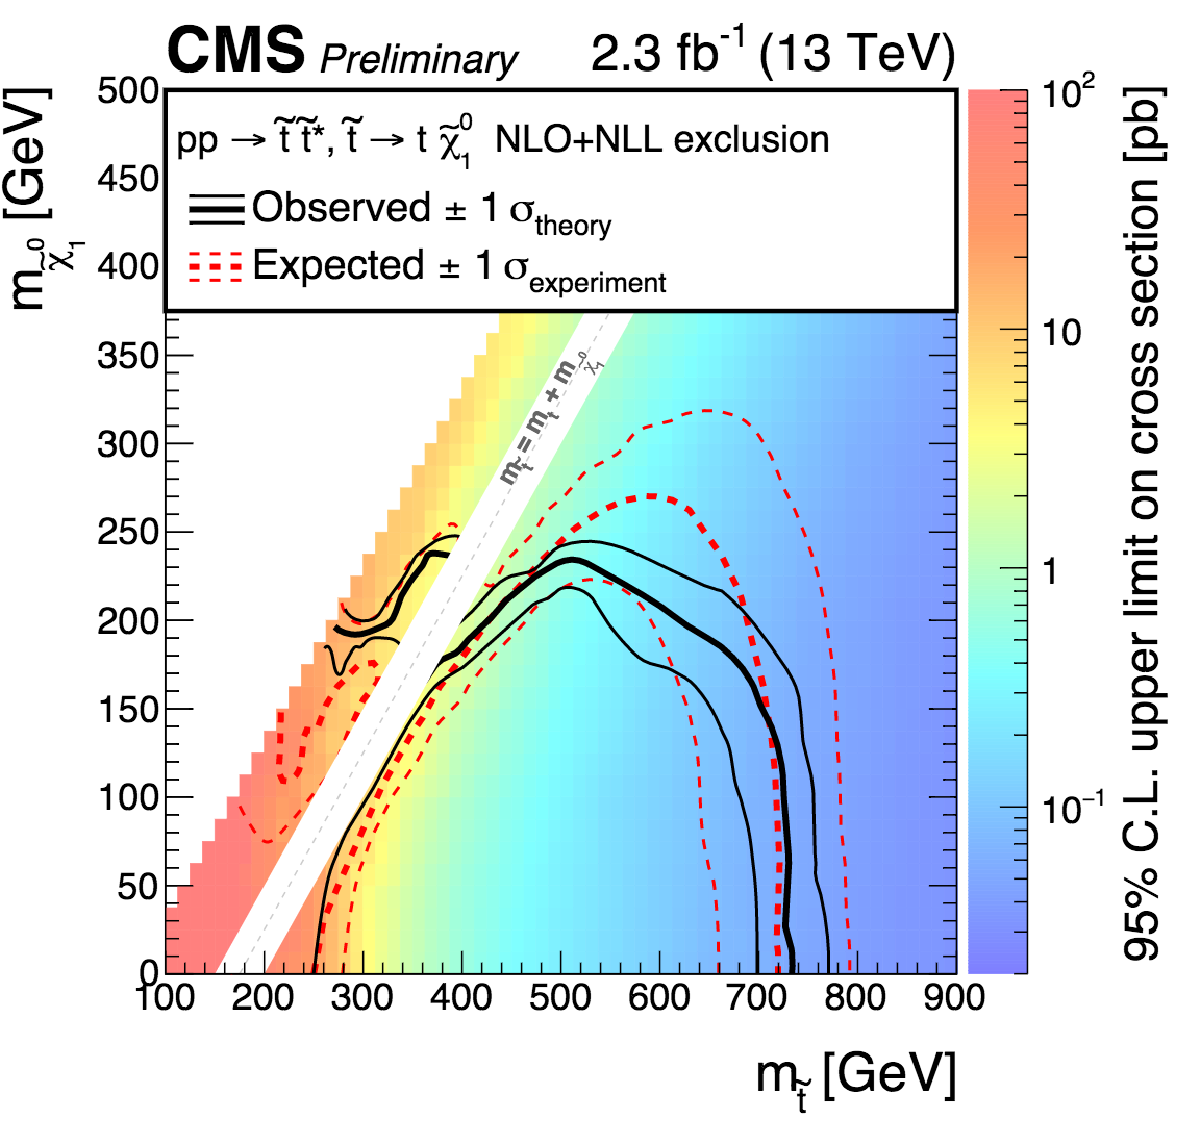
\includegraphics[width=0.4\textwidth]{1lstop/T2tt_limits.pdf}
%% \end{tabular}
%% \caption{
%% \label{fig:1lstopresults}
%% Observed yields and background predictions are shown for the 1 lepton stop analysis on the left,
%% and the cross section upper limit set by these results is shown on the right.
%% }
%% \end{center}
%% \end{figure}

The next analysis is a search targeting final states with exactly one lepton~\cite{1lmj2015}, and many jets from hadronic top decay.
In this analysis, events with exactly 1 lepton in the final state are selected,
and the jets in the event ($\mathrm{R=0.4}$) are reclustered to form large-R jets ($\mathrm{R=1.2}$).
The mass of these large-R jets is then summed to form the variable \MJ\
which tends to be large for events where large mass particles decay hadronically, for example in SUSY in final states with many top quarks.
The results of this analysis are interpreted in the context of a SUSY model where gluinos are pair-produced then each decays to a \ttbar\ pair and a stable LSP,
and gluinos up to a mass of 1600 GeV are excluded.

%% \begin{figure}[!htb]
%% \begin{center}
%% \begin{tabular}{cc}
%% 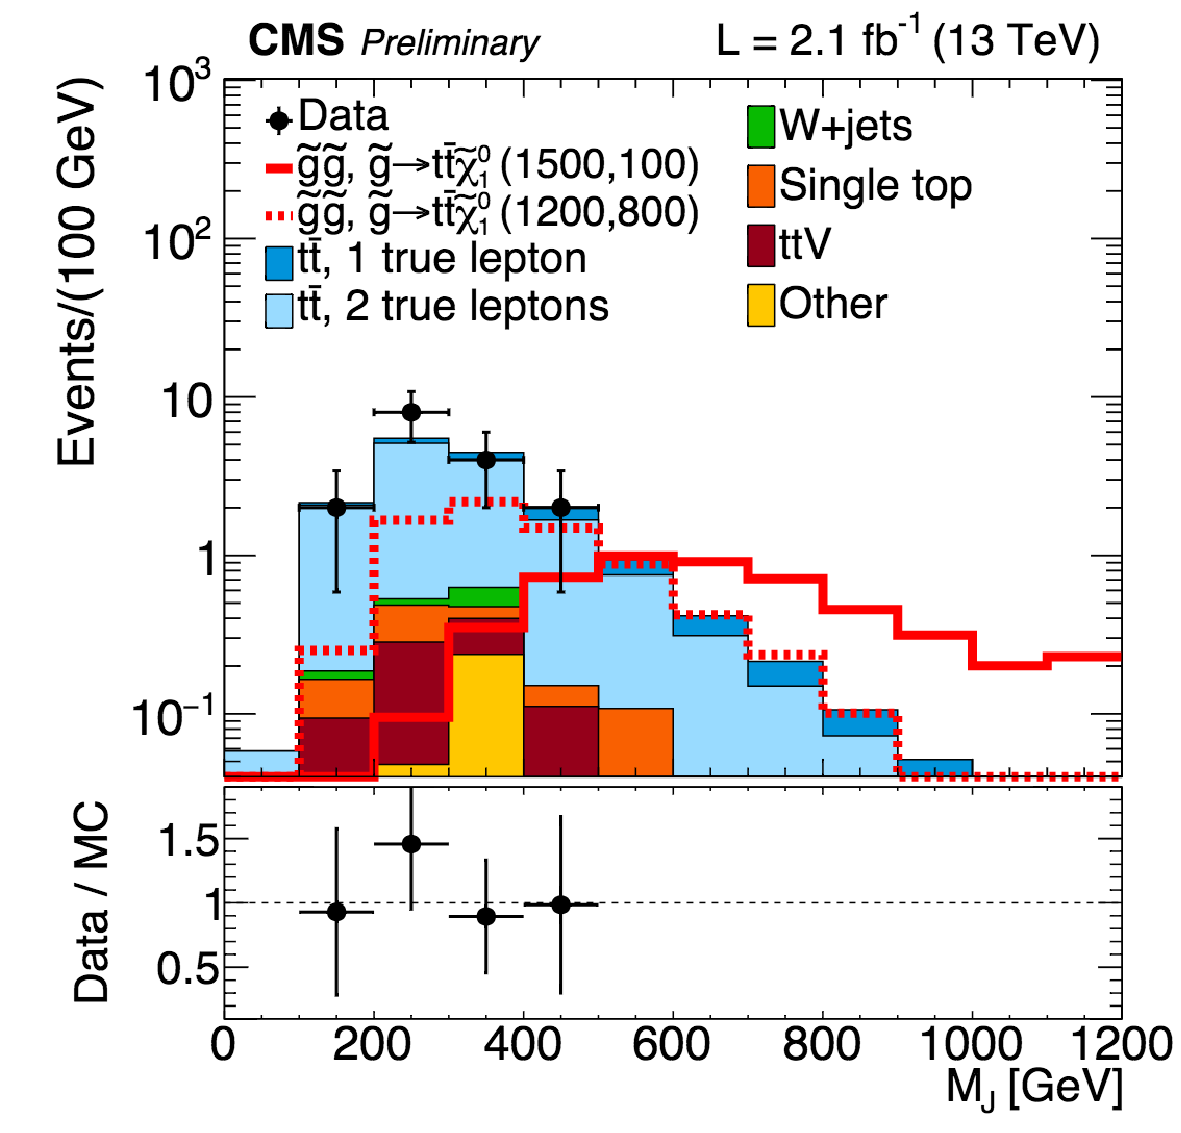
\includegraphics[width=0.4\textwidth]{1lmjet/MJ.pdf} &
%% 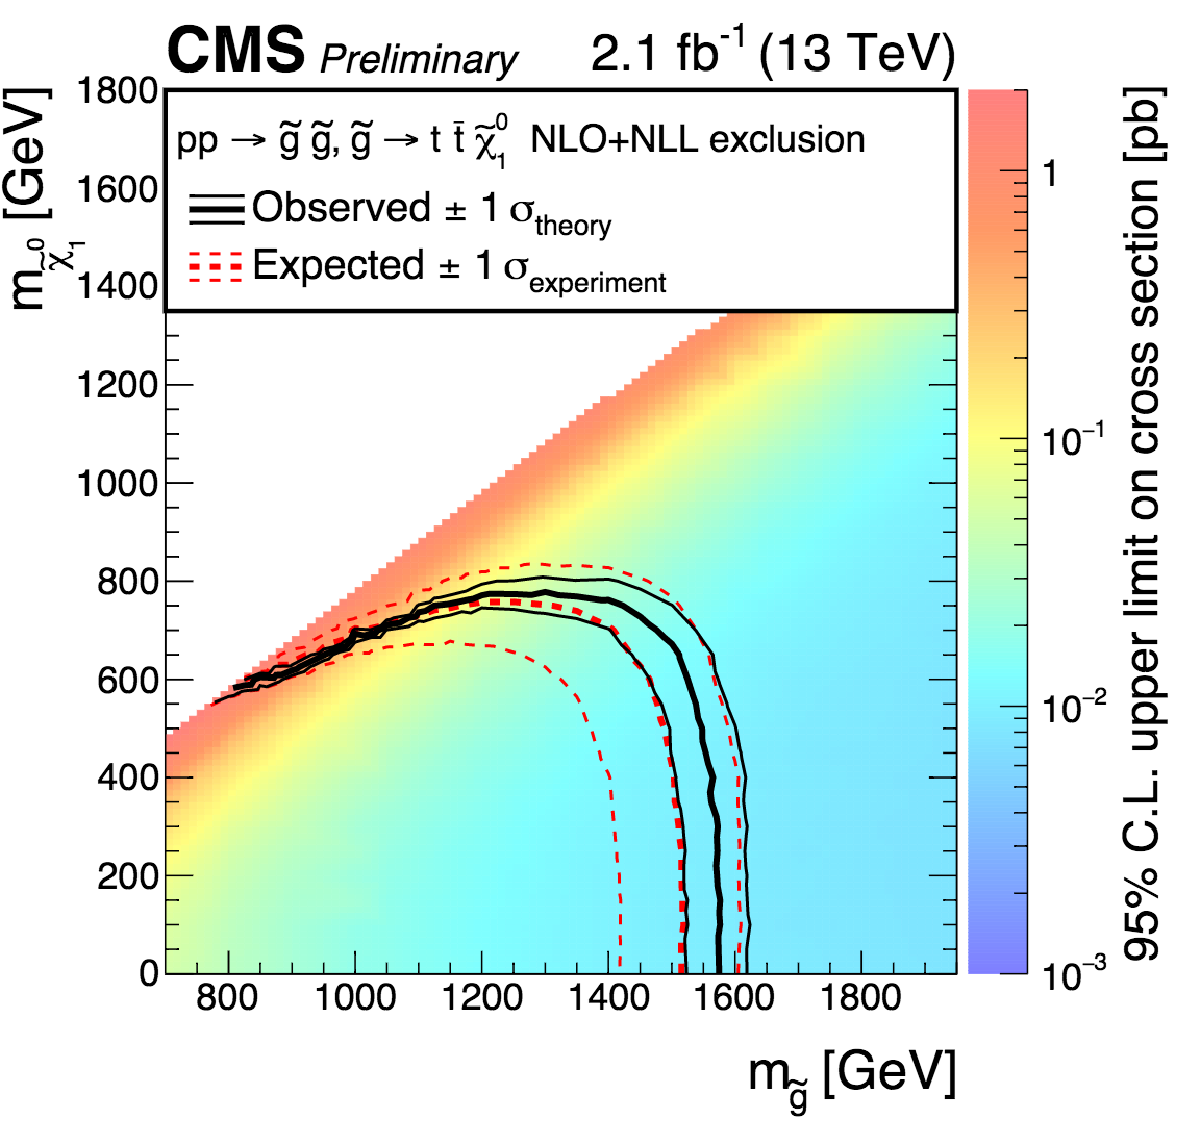
\includegraphics[width=0.4\textwidth]{1lmjet/T1tttt_limits.pdf}
%% \end{tabular}
%% \caption{
%% \label{fig:1lmjetresults}
%% Observed yields and background predictions are shown for the \MJ\ analysis on the left,
%% and the cross section upper limit set by these results is shown on the right.
%% }
%% \end{center}
%% \end{figure}


The final analysis with exactly one lepton~\cite{1lincl2015} is an inclusive search
which uses the \dphiwl\ and \LT\ variables to suppress SM backgrounds which mostly consist of \ttbar\ and W+jets.
These variables are shown in figure~\ref{fig:1linclresults} for the signal region where events with a b-tagged jet are vetoed.
The search is binned in the variables HT, njets, nb-tags in order to maximize sensitivity to new physics.
The results of the search are interpreted many SUSY scenarios, for example the same model as the \MJ\ analysis,
and this analysis is seen to have similar sensitivity when interpreting the results within the context of this simplified model.

\begin{figure}[!htb]
\begin{center}
\begin{tabular}{cc}
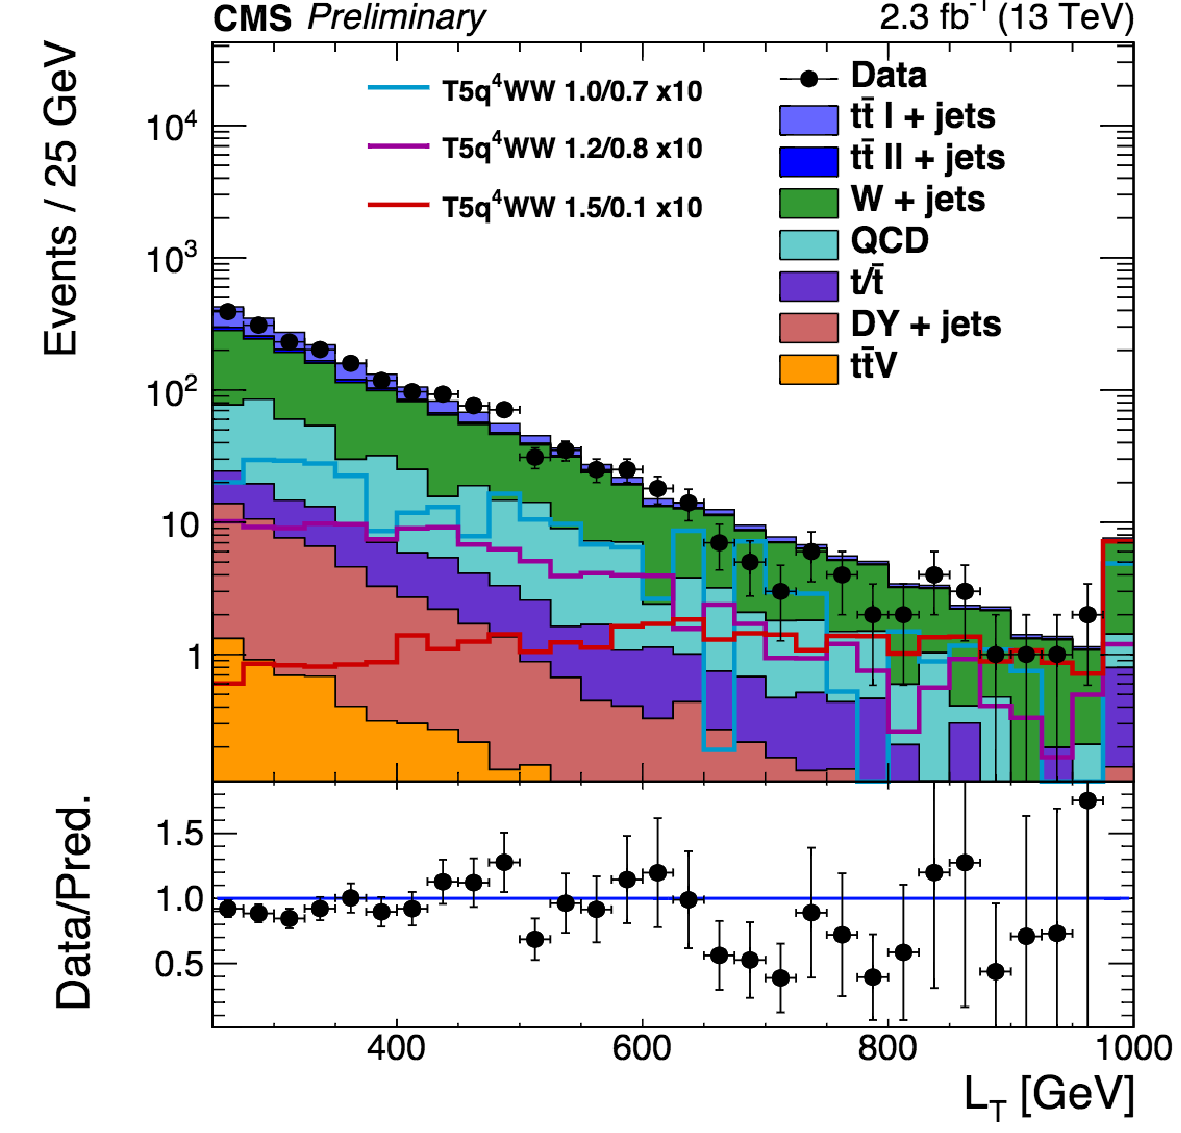
\includegraphics[width=0.4\textwidth]{1lincl/LT.pdf} &
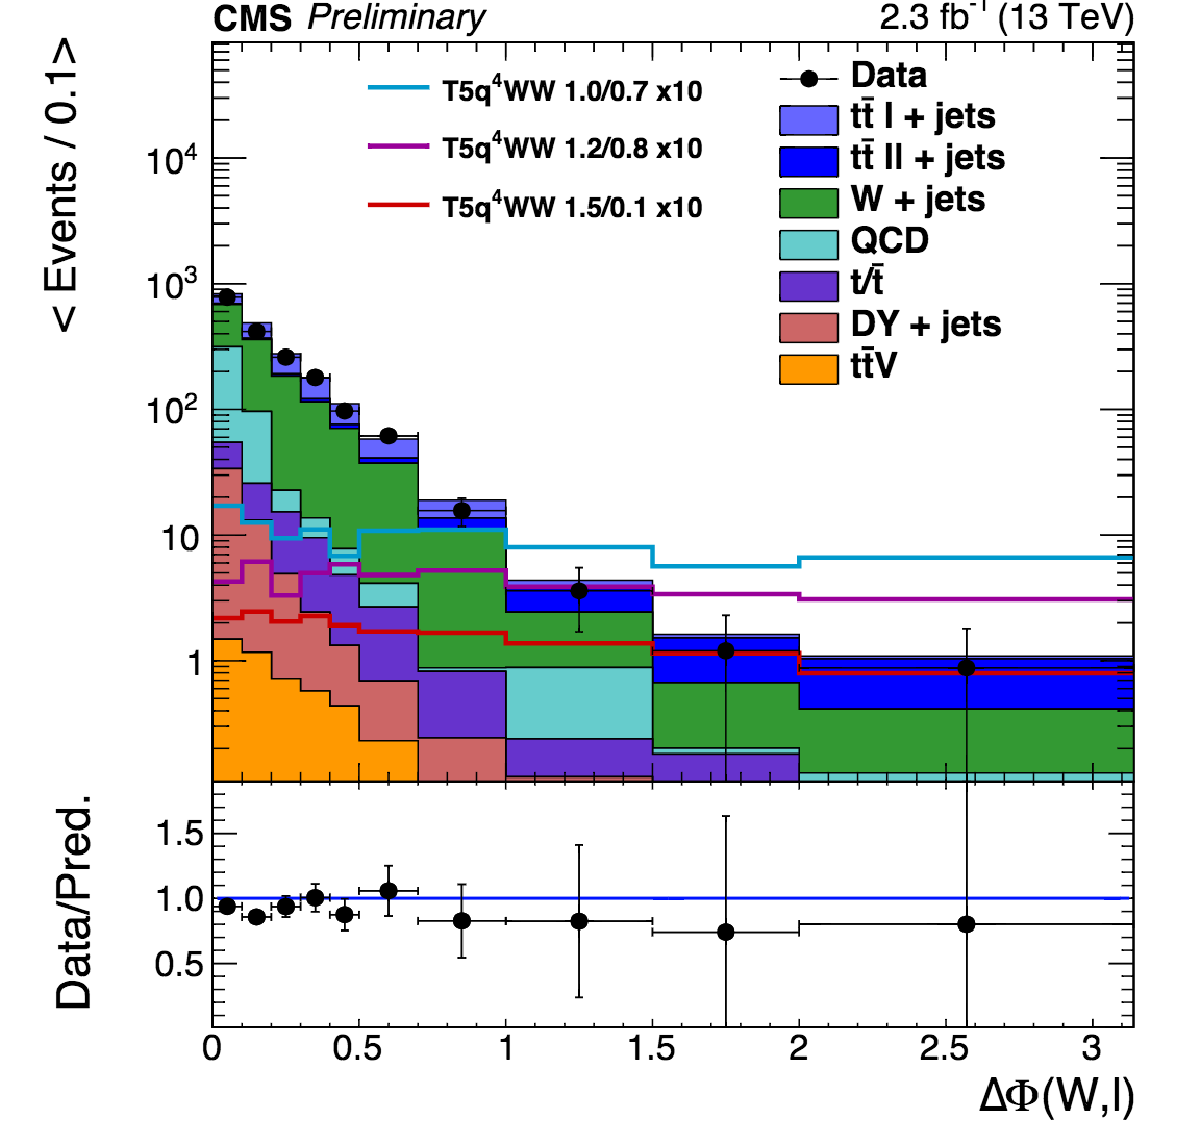
\includegraphics[width=0.4\textwidth]{1lincl/dphiWl.pdf}
\end{tabular}
\caption{
\label{fig:1linclresults}
Observed yields and background predictions are shown for the inclusive 1-lepton analysis
for the variables \LT\ (left) and \dphiwl\ (right).
}
\end{center}
\end{figure}

